% preamble and style file for M&R lecture slides
\documentclass[11.5pt,sans,english]{beamer}

\usetheme{EastLansing}
\usecolortheme{lily}

\usepackage[most]{tcolorbox}

\usepackage{verbatim}
%\usepackage{ulem}
%\usepackage{fontawesome}
%\usepackage{tikz}
%\usepackage{pifont}
%\usepackage{tabularx}
\usepackage{array,booktabs,xcolor,colortbl,multirow,rotating,amssymb}
%\usepackage{amsmath}
% \usepackage{vwcol}
% \usepackage[T1]{fontenc}

  
\newcommand\vect[1]{\underline{\mathbf{#1}}}
\newcommand\unitvect[1]{\hat{\boldsymbol{#1}}}
%\newcommand\hatdot[1] { \hat{ \dot{ \boldsymbol{#1} } } }

\newtcbox
{\keyc}{on line,arc=2pt, colback=yellow!30!white, colframe=yellow!30!black, before upper={\rule[-3pt]{0pt}{10pt} },boxrule=1pt,boxsep=0pt,left=6pt,right=6pt,top=2pt,bottom=2pt,}

\newtcbox
{\keyb}{on line,arc=1pt, colback=blue!30!white, colframe=blue!30!black, before upper={\rule[-3pt]{0pt}{10pt} },boxrule=1pt,boxsep=0pt,left=6pt,right=6pt,top=2pt,bottom=2pt,}

\newtcbox
{\keyl}{on line,arc=1pt, colback=pink!30!white, colframe=blue!30!black, before upper={\rule[-3pt]{0pt}{10pt} },boxrule=1pt,boxsep=0pt,left=6pt,right=6pt,top=2pt,bottom=2pt,}

\newtcbox
{\keyw}{on line,arc=1pt, colback=red!30!white, colframe=blue!30!black, before upper={\rule[-3pt]{0pt}{10pt} },boxrule=1pt,boxsep=0pt,left=6pt,right=6pt,top=2pt,bottom=2pt,}

\newtcbox
{\keya}{on line,arc=1pt, colback=purple!30!white, colframe=blue!30!black, before upper={\rule[-3pt]{0pt}{10pt} },boxrule=1pt,boxsep=0pt,left=6pt,right=6pt,top=2pt,bottom=2pt,}

\newtcbox[auto counter,number within=section]
{keyf}
{
enhanced,
on line,
  boxsep=0pt,
  left=6pt,right=6pt,top=2pt,bottom=2pt,
  arc=5pt,
  boxrule=1pt,
  rightrule=38pt,
colback=green!10!white, 
colframe=green!50!black, 
title=\thetcbcounter,
detach title,
overlay unbroken and first ={
    \node[%rotate=90,
          %minimum width=1cm,
          anchor=south,
          font=\sffamily\bfseries\tiny,
          %yshift=-10pt,
          yshift=-5pt,
          xshift=-20pt,
          white]
    at (frame.east) {\thetcbcounter};
  }
}


\usepackage{xcolor}

%\usepackage{hyperref}
%\hypersetup{
%  pdfauthor={Lily Asquith},
%  urlcolor=blue,
%  colorlinks=true,
%  linkcolor=blue,
%  bookmarks=true
%}

%---------------------------------------------%
%              LILY'S COLOURS           %
%---------------------------------------------%
\definecolor{Wash}{RGB}{204,204,204}
%\definecolor{Pinky}{RGB}{254,200,254}%violet
\definecolor{Pinky}{RGB}{219,	240,	253}%violet
\definecolor{Bluey}{RGB}{0,190,255}%deep sky blue
\definecolor{DarkGrey}{RGB}{28,66,137}%dar grey
\definecolor{SussexWhite}{RGB}{253,255,254}%dar grey
\definecolor{LightGray}{RGB}{184,184,255}
\definecolor{YesGreen}{RGB}{0,128,0}
\definecolor{NoRed}{RGB}{250,0,0}



\definecolor{myred}{RGB}{255,153,153}
\definecolor{myorange}{RGB}{255,204,153}
\definecolor{myyellow}{RGB}{255,255,153}
\definecolor{mygreen}{RGB}{153,255,153}
\definecolor{mycyan}{RGB}{153,255,255}
\definecolor{myblue}{RGB}{153,204,255}
\definecolor{myviolet}{RGB}{153,153,255}
\definecolor{mypurple}{RGB}{204,153,255}
\definecolor{mypink}{RGB}{255,204,255}
\definecolor{mycoral}{RGB}{255,153,204}

%-----------------------------------------------------%
%              LILY'S COLUMN TYPES          %
%-----------------------------------------------------%
\newcolumntype{a}{>{\raggedright\arraybackslash}l}	
\newcolumntype{q}{>{\raggedright\arraybackslash}m{8cm}} 

%--------------------------------------------%
%              LILY'S SYMBOLS          %
%--------------------------------------------%
\newcommand{\dfinger}{\large{\textcolor{black}{\ding{43}}}\scriptsize}
\newcommand{\dstar}{\large{\textcolor{black}{\ding{76}}}\scriptsize}
\newcommand{\dwrite}{\large{\textcolor{black}{\ding{45}}}\scriptsize}
\newcommand{\ddiamond}{\small{\textcolor{DarkGrey}{\ding{117}}}\scriptsize}
\newcommand{\ddiamondwhite}{\small{\textcolor{SussexWhite}{\ding{117}}}\scriptsize}
\newcommand{\experiment}{\small{\textcolor{magenta}{\faCogs }}\scriptsize}
\newcommand{\watchit}{\textcolor{blue}{ \faYoutube}}


\makeatletter
\newcommand\notsotiny{\@setfontsize\notsotiny{6.5}{7.5}}
\makeatother


% 
\title[ Mechanics \& Relativity]{Mechanics \& Relativity}
\subtitle{\textbf{Topic 1: Kinematics }}
\author[Dr Lily Asquith (Lily)]{ Dr Lily Asquith (Lily)}
\date[28-30 September 2021]{28-30 September 2021 (Week 1)}
\logo{

\includegraphics[width=1.5cm]{../../utils/uslogo.jpg}
}


\begin{document}


\begin{frame}
\titlepage
\end{frame} 

 %-----------------------------------------------------------%
 % 1 Kinematics                                                 %
 %-----------------------------------------------------------%
\section{M\&R 1: Kinematics}
\begin{frame}
\frametitle{Kinematics} 
\normalsize

This week's topics:\\[3ex]

\begin{itemize}
\item[1.1] Displacement, Velocity \& Acceleration\\[3ex]
\item[1.2] Equations of motion (SUVAT)\\[3ex]
\item[1.3] Reading graphs\\[3ex]
\end{itemize}
\end{frame} 
 
 %-----------------------------------------------------------%
 % LECTURE 1
 %-----------------------------------------------------------%
 
 \subsection{Displacement, Velocity \& Acceleration }

%  
\begin{frame}{Notation}
$s$ : for position (or sometimes $x$, or $y$, or $r$...)\\
%$\vect{s}$ or $\vec{s}$ : for linear displacement with a direction\\
$u$ : for (magnitude of) initial velocity (aka initial speed)\\
$v$ : for (magnitude of) velocity (aka speed)\\
%$\vect{v}$ or $\vec{v}$ : for speed with a direction (velocity)\\
$a$ : for (magnitude of) acceleration\\
%$\vect{a}$ or $\vec{a}$ : for acceleration with a direction\\
$t$ : for time (\textcolor{blue}{is time a vector?})\\[1ex]
$\Delta$ : means \textit{`change in'} \\[1ex]
$\delta$ or $d$ : means \textit{`teeny weeny change in'} \\[1ex]

Standard units of displacement in space and time are metres and seconds, unless otherwise stated.\\

\end{frame}
 
% 
\begin{frame}{Displacement}
\small
To begin to talk about where something is, let alone where it is headed, we need three things:
\begin{itemize}
\item[1]  A coordinate system, $eg$ cartesian coordinates (x, y, z).
\item[2]  A reference point: \textbf{the origin}.\\[1ex]
\item[3]  A positive direction.\\[1ex]
\end{itemize}

\begin{center}
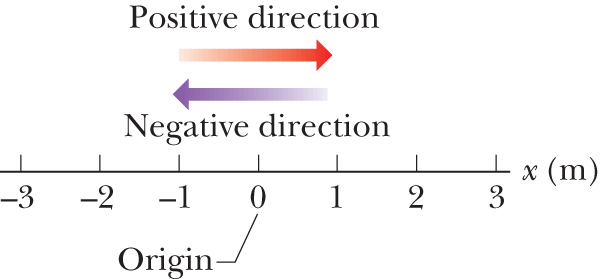
\includegraphics[scale=0.8]{1.png}
\end{center}

We can then define the displacement as \textbf{ the change in position:} \\[1ex]

\keyf{ $\Delta s = s_{f} - s_{i}$}  

\end{frame}
 
 \begin{frame}{Poll everywhere checkpoint }
 Here are three pairs of initial and final positions: [$s_i, s_f$] along an x axis. Which pairs give a \textit{negative displacement $\Delta s$}?\\[1ex]
 (a) [-3 m, +5 m]\\ 
 (b) [-3 m, -7 m]\\
 (c) [7 m, -3 m]\\[3ex]

\fbox{\begin{minipage}{\textwidth}
Use your phone to go to: \textcolor{blue}{pollev.com/ilovephysics} and select the option:\\
 A :  a \& b give negative displacements\\
 B :  a \& c   \\
 C :  b \& c 
 \end{minipage}}
 \vspace{0.5cm}
 
 Don't panic, these polls are always anonymous!
 
 
 \end{frame}
 
 % 
\begin{frame}{Displacement}
An object may be motionless in space, but it will always move through time.\\[2ex]
\centering
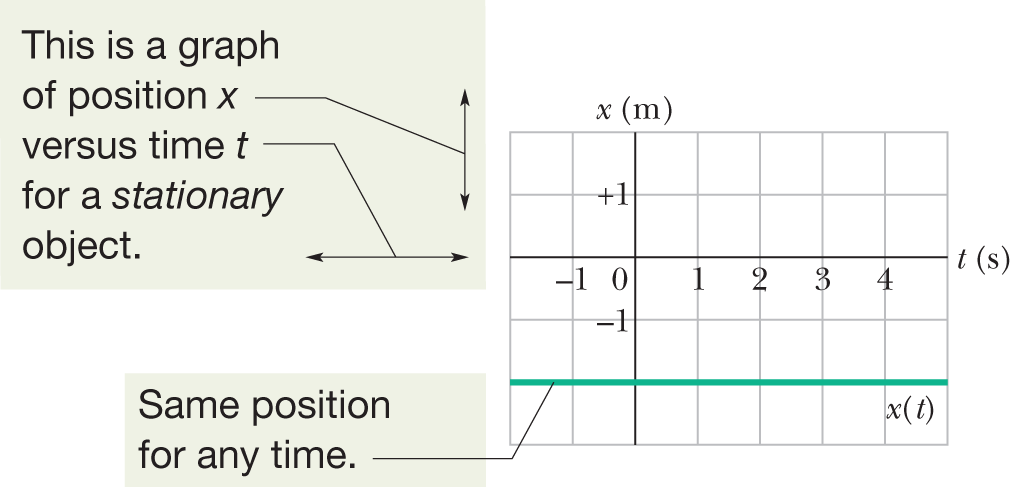
\includegraphics[scale=1.]{2.png}
\end{frame}


% 
\begin{frame}{Average velocity}
To find the average velocity, we divide the total distance by the total time.\\[2ex] 
\centering
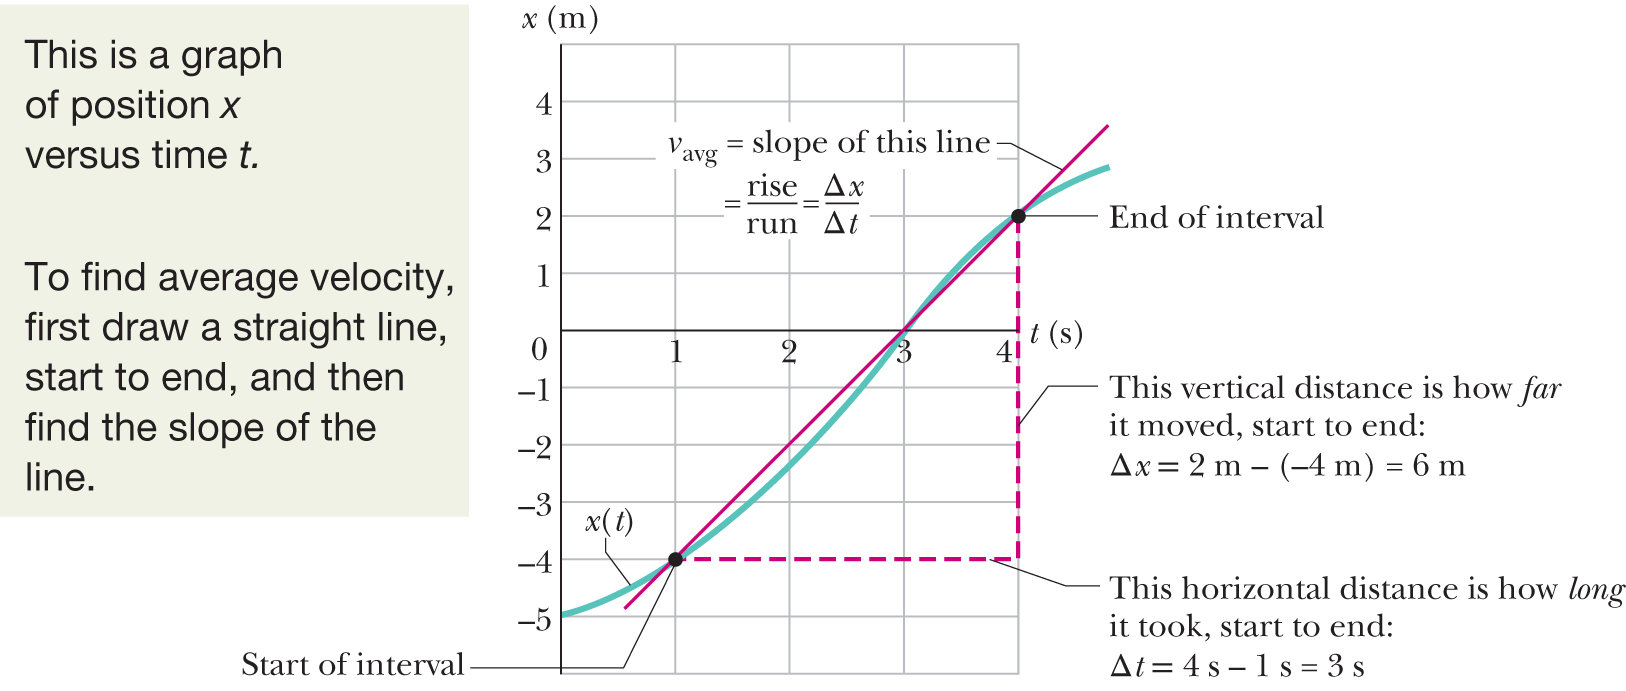
\includegraphics[scale=0.8]{3.png}
\end{frame}


%   
\begin{frame}{Solving a problem of this sort}
\small
You drive along a straight road for 8.4 km at 70 km/h, at which point your car runs out of petrol and stops. Over the next 30 min, you walk another 2.0 km along the road to a petrol station.\\[1ex]
\textit{What are your overall displacement, time taken, and average speed from the beginning of your drive to your arrival at the station?}\\[1ex]

\vspace{5cm}
\end{frame}

 
 %  
\begin{frame}{Instantaneous velocity}

We can define the velocity (and acceleration) either as average or as instantaneous.\\[2ex]

The average velocity and acceleration over a period of time given by $\Delta t$ is: \\[2ex]
\keyf{$\vect{v}_{avg} = \frac{\Delta \vect{s} }{\Delta t} $; \;\; $\vect{a}_{avg} = \frac{\Delta \vect{v} }{\Delta t} $} \\[2ex]

The instantaneous velocity and acceleration  at an exact moment in time is: \\[2ex]
\keyf{$\vect{v} = \frac{\delta  }{\delta t} \vect{s}$; \;\; $\vect{a} = \frac{\delta  }{\delta t} \vect{v}= \frac{\delta^2  }{\delta t^2} \vect{s}$} \\[1ex]
\end{frame}



%  
\begin{frame}{A bit more notation / reminder of calculus...}

$\frac{d s }{d t} $: the differential of position With Respect To (wrt) time.\\[1ex]
$\frac{d^2 s }{d t^2} $ : the second differential of position wrt time.\\[3ex]

Example \& Notation: \\[10ex]






\end{frame}

 
  \begin{frame}{Checkpoint }
  \small
The following equations give the position $x(t)$ of a particle in four situations (in each equation, $x$ is in meters, $t$ is in seconds, and $t > 0$):\\[2ex]

 (1) $x = 3t - 2$\\[1ex]
 (2) $x = -4t^2 - 2$\\[1ex]
 (3) $x = \frac{2}{t^2}$\\[1ex]
 (4) $x = -2$ \\[3ex]
 
%\fbox{\begin{minipage}{\textwidth}
%Use your phone to go to: \textcolor{blue}{pollev.com/ilovephysics}
 (a) In which situation(s) is the velocity v of the particle constant? \\[2ex]
 (b) In which is v in the negative x direction?\\
%\end{minipage}}
\vspace{2cm}
 
 
 \end{frame}
 
 %  
\begin{frame}{Acceleration}
\small
Acceleration usually means `speeding up' in normal conversation. In physics it also means `slowing down'.\\[1ex]

If something has a changing speed, then its acceleration is non-zero\\[1ex]

Which of these positions as a function of time correspond to constant acceleration?\\[1ex]
$x = 4t^3 - 55$:\\[1ex]
$x = 4t^2 - 55$:\\[1ex]
$x = 4t - 55$:\\[1ex]
$x = 4/t - 55$:\\[1ex]
$x = 4/t^2 - 55$:\\[1ex]
%$x = 4/t^3 - 55$:\\[1ex]
\end{frame}


\begin{frame}{Before next lecture}

Retry the pre-lecture quiz 1.1  Velocity and Acceleration, if you like.\\[2ex]
Attempt the pre-lecture quiz for 1.2  Equations of Motion.\\[2ex]
See you tomorrow morning for lecture 1.2\\

\end{frame}

%-----------------------------------------------------
%     LECTURE 2
%-----------------------------------------------------

\subsection{Equations of Motion for constant acceleration}
\begin{frame}{suvat}
$s$ : for position \\
%$\vect{s}$ or $\vec{s}$ : for linear displacement with a direction\\
$u$ : for (magnitude of) \textbf{initial} velocity (aka initial speed)\\
$v$ : for (magnitude of) velocity (aka speed)\\
%$\vect{v}$ or $\vec{v}$ : for speed with a direction (velocity)\\
$a$ : for (magnitude of) acceleration\\
%$\vect{a}$ or $\vec{a}$ : for acceleration with a direction\\
$t$ : for time \\[1ex]

We will consider situations where displacement $s$ and velocity $v$ are functions of time $t$.\\[1ex]

\textcolor{red}{We cannot use suvat for situations where the acceleration is not constant.}\\[1ex]

It is convenient to memorise certain formulae for calculating one of these things when others are known, such as \\[1ex]

 $\vect{v} = \vect{u} + \vect{a}t$ \\[1ex]

But where does this come from?

\end{frame}



\begin{frame}{How do we know v= u + at ?}
\small
The first equation of motion for translational motion is derived starting from the definition for acceleration as the change in velocity with time:\\[1ex]

\textcolor{blue}{$\displaystyle \vect{a} $} = \textcolor{red}{$\displaystyle \frac{d}{dt}\vect{v}$} $\rightarrow \;$  \textcolor{blue}{$\displaystyle \int \vect{a} dt$} = \textcolor{red}{$ \displaystyle \int \frac{d}{dt}\vect{v} dt$} $\rightarrow \; $\textcolor{blue}{$\vect{a}t + \vect{c}$} = \textcolor{red}{$ \vect{v} $}\\[1ex]

\keyc{We can write  $ \int \vect{a} dt = \vect{a}t$ because $a$ is constant: not a function of time.}\\[1ex]

We find the constant of integration $\vect{c}$ by setting $t = 0 \rightarrow \vect{c} = \vect{v}_0 .$\\[2ex]

This gives us $\vect{a}t + \vect{v}_0 = \vect{v}$, which is often reorganised as\\[1ex]
\keyf{ $\vect{v} = \vect{u} + \vect{a}t$}  
 where we are now using $\vect{v}_0 \rightarrow \vect{u}$ for the \textbf{initial velocity}.\\[1ex]




\keyc{This equation contains no $\vect{s}$, so we use it when $\vect{s}$ is unknown and unwanted}\\[1ex]
\vspace{1cm}

\end{frame}


%---------------%
% EQNS OF MOTION : SUVAT 2
%---------------%
\begin{frame}{ How about $s = ut + \frac{1}{2}at^2$ ?}
\small
The second equation of motion is derived starting from the definition for velocity:\\[1ex]

\textcolor{blue}{$\displaystyle \vect{v} $} = \textcolor{red}{$\displaystyle \frac{d}{dt}\vect{s}$} $\rightarrow \;$  \textcolor{blue}{$\displaystyle \int \vect{v} dt$} = \textcolor{red}{$ \displaystyle \int \frac{d}{dt}\vect{s} dt$} \\[1ex]
%$ v = \frac{ds}{dt} \rightarrow  \displaystyle \int v dt  = \displaystyle \int \frac{ds}{dt} dt$\\[1ex]
Now we have to substitute for $\vect{v} = \vect{u}+\vect{a}t$ (suvat 1) in the LHS because unlike $\vect{a}$ (which has to be constant for these equations to work) $\vect{v}$ \textbf{can be a function of time}:\\[1ex]

 \textcolor{blue}{$\displaystyle \int (\vect{u} + \vect{a}t) dt$} = \textcolor{red}{$ \displaystyle \int \frac{d}{dt} \vect{s} dt$} $\rightarrow \;$  \textcolor{blue}{$\vect{u}t + \frac{1}{2}\vect{a}t^2 + \vect{c}$} = \textcolor{red}{$\vect{s}$} \\[1ex]


We find the constant of integration $\vect{c}$ by setting $t = 0 \rightarrow \vect{c} = \vect{s}_0 $\\[1ex]

This gives us $\vect{u}t + \frac{1}{2}\vect{a}t^2 + \vect{s}_0 = \vect{s}$, which is often reorganised as \\[1ex]
\keyf{$\vect{s} = \vect{u}t + \frac{1}{2}\vect{a}t^2$}  
where we are now using $\vect{s}_0 =0$ for the initial position.\\[1ex]

\keyc{This equation contains no $\vect{v}$, so we use it when $\vect{v}$ is unknown and unwanted}\\[1ex]
\end{frame}


\begin{frame}{ Eliminating The Unknowns  : \textit{\textcolor{red}{I don't know $a$ !} }}
\small


\begin{columns}[T]
\begin{column}{0.7\textwidth}
 Eliminate $a$ by rearranging [1]: $\textcolor{red}{a}= \textcolor{blue}{ (v-u) / t}$\\[1ex]
Sub into [2]: 
\begin{equation}\nonumber
\begin{split}
s  &= ut + \frac{1}{2} [\textcolor{blue}{(v-u) / t}] t^2  \\
& = ut + \frac{1}{2} [(v-u)] t \\
\end{split}
\end{equation}
\end{column}\hfill

\begin{column}{0.3\textwidth}

        
\keyl{$v= u + at$ [1]} \\[1ex] 
\keyl{$s = ut + \frac{1}{2}at^2$ [2] } \\[3ex] 
\end{column}
\end{columns}
\vspace{0.5cm}

\keyf{$s= \frac{1}{2} (v+u) t$}.  \keyc{contains no $a$, so we use it when $a$ is unknown}\\[1ex]

\end{frame}


\begin{frame}{ Eliminating The Unknowns  : \textit{\textcolor{red}{I don't know $t$ !} }}
\small
\begin{columns}[T]
\begin{column}{0.7\textwidth}
 Eliminate $t$ by rearranging [1]: $\textcolor{red}{t}= \textcolor{blue}{ (v-u) / a}$\\[1ex]
Sub into [2]: 
\notsotiny
\begin{equation}\nonumber
\begin{split}
s &= u  [\textcolor{blue}{ (v-u) / a}]+ \frac{1}{2} a [\textcolor{blue}{ (v-u) / a}]^2  \\
   &= uv/a -u^2/a + \frac{1}{2} a (v^2 + u^2 -2uv) / a^2 \\
  &= uv/a -u^2/a + \frac{1}{2} v^2/a +  \frac{1}{2}u^2/a - \frac{1}{2}2uv)/a \\
 & = -u^2/a + \frac{1}{2} v^2/a +  \frac{1}{2}u^2/a\\[1ex]
\end{split}
\end{equation}
\end{column}\hfill

\begin{column}{0.3\textwidth}
       
\keyl{$v= u + at$ [1]} \\[1ex] 
\keyl{$s = ut + \frac{1}{2}at^2$ [2] } \\[3ex] 
\end{column}
\end{columns}

\vspace{0.5cm}

\keyf{$s =  \frac{1}{2} (v^2 +u^2)/a$}  \keyc{contains no $t$, so we use it when $t$ is unknown}\\[1ex]



\end{frame}



\begin{frame}{ Eliminating The Unknowns  : \textit{\textcolor{red}{I don't know $u$ !} }}
\small

\begin{columns}[T]
\begin{column}{0.7\textwidth}
Eliminate $u$ by rearranging [1]: $\textcolor{red}{u}= \textcolor{blue}{ v - at}$\\[1ex]
Sub into [2]: 
\begin{equation}\nonumber
\begin{split}
s  &= [\textcolor{blue}{ v - at}] t + \frac{1}{2} at^2  \\
& = vt - at^2 + \frac{1}{2} at^2 \\
\end{split}
\end{equation}
\end{column}\hfill

\begin{column}{0.3\textwidth}
       
\keyl{$v= u + at$ [1]} \\[1ex] 
\keyl{$s = ut + \frac{1}{2}at^2$ [2] } \\[3ex] 
\end{column}
\end{columns}

\vspace{0.5cm}
\keyf{$s = vt -  \frac{1}{2}at^2 $}  \keyc{contains no $u$, so we use it when $u$ is unknown}\\[1ex]

\end{frame}


%\begin{frame}{Solving a problem of this sort}
%\small
%You are driving toward a traffic light when it turns yellow. Your speed is the legal speed limit of $v_0 = 55$ km/h; your best deceleration rate has the magnitude $a = 5.18$ ms$^{-2}$. Your best reaction time to begin braking is $t = 0.75$ s. To avoid having the front of your car enter the junction after the light turns red, should you brake to a stop or continue to move at 55 km/h if the distance to the intersection and the duration of the yellow light are:\\[1ex]
% (a) 40 m and 2.8 s\\[1ex]
% (b) 32 m and 1.8 s\\[1ex]
% 
% Give an answer of brake, continue, either (if either strategy works), or neither (if neither strategy works and the yellow duration is inappropriate).\\[10ex]
%
%
%\end{frame}

\begin{frame}{Freefall Acceleration}
\small
We will talk about gravity later. For now: \\[1ex]

Acceleration due to gravity $g = -9.81 ms^{-2}$\\[1ex]

This is an approximation: $g$ actually varies. But we treat it as a constant, and it is \textbf{constant wrt to time}.\\[1ex]

For problems on and near the Earth's surface, we can use $g$ for $a$ in suvat: handy.\\[3ex]

The fastest creature on earth is supposedly the Peregrine Falcon, which can `fly' (actually dive) at 389 kmh$^{-1}$.\\[1ex]

What is this in ms$^{-1}$?\\[6ex]

%$389 km/h = 3.89\times10^2 km/h = 3.89\times10^5 m/h = 3.89\times10^5 m / 3600 s =108 m/s $\\
\end{frame}



\begin{frame}{Freefall Acceleration}
\small
How fast could I `fly' if dropped from a height of 1km?\\

$u = 0$ ms$^{-1}$\\
$s = 10^3$ m\\
$a = -9.81$ ms$^{-2}$\\

Which variable is both unknown and unwanted?\\[2ex]

$s =  \frac{1}{2} (v^2 +u^2)/a$\\
$2as =  v^2 +u^2$\\
$v = \sqrt{2as - u^2}$\\
$|v| = \sqrt{2*9.81*1000} = 140 m/s$\\

So why am I not listed on wikipedia as the fastest creature on Earth?


%https://en.wikipedia.org/wiki/Fastest_animals
\end{frame}






\begin{frame}{Solving a problem of this sort}
\small
A car traveling 56.0 kmh$^{-1}$ is 24.0 m from a barrier when the driver slams on the brakes. The car hits the barrier 2.00 s later. \\[1ex]

(a) What is the magnitude of the car's constant acceleration before impact? \\[10ex]
(b) How fast is the car traveling at impact?\\[6ex]
\end{frame}



%
%\begin{frame}{Cheetah versus sports car}
%
%\href{https://www.youtube.com/watch?v=8-9oFxYFODE}{https://www.youtube.com/watch?v=8-9oFxYFODE}
%
%
%Cheetah fasted speed: 105 km/h,  highest acceleration: 10 m/s$^2$. 0 to 96.6 km/h in 3s. Max t 60 s\\
%Lily's car 180 km/h, goes 0 to 180 km/h  in 52.8 sec\\
%
%
%\end{frame}






\begin{frame}{If there is no air resistance}

In the absence of any external forces, all objects fall towards the centre of the planet with $a = g =9.81$ ms$^{-2}$.\\[1ex]

This can seem \textit{counter-intuitive} because it is something we can almost never observe.\\[1ex]

We are all accelerating at $g$ right now. The normal force of the Earth is matching that acceleration in the opposite direction.\\[1ex]

Could I accelerate at $g$ forever, if there were no atmosphere or other stars, planets?\\[1ex]


\end{frame}



\begin{frame}{Poll Everywhere Checkpoint}

You are standing on a bridge with two eggs. You drop one, and you throw the other directly downwards.\\

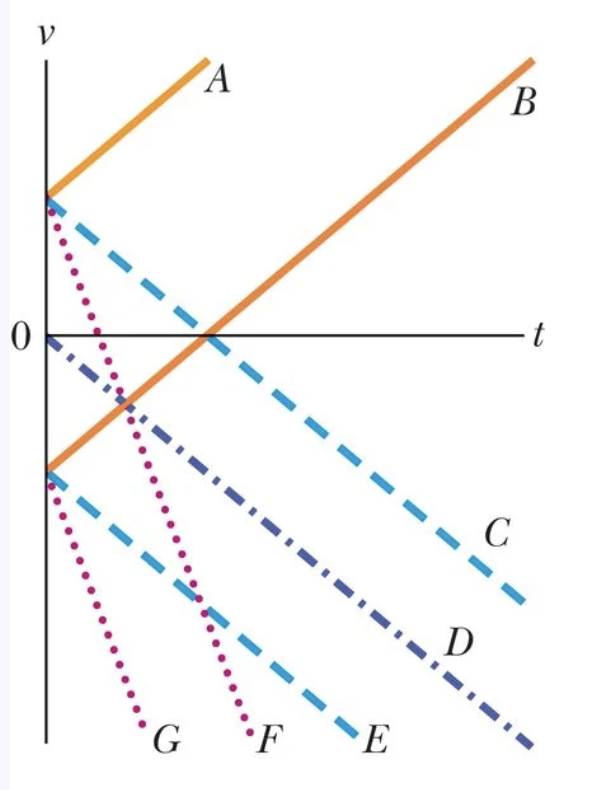
\includegraphics[scale=0.3]{vt-graph}
 
\fbox{\begin{minipage}{\textwidth}
Use your phone to go to: \textcolor{blue}{pollev.com/ilovephysics}\\
 (a) Which line best describes the motion of the dropped egg? \\
 (b) Which line best describes the motion of the thrown egg?\\
\end{minipage}}
\vspace{2cm}

\end{frame}



\begin{frame}{Before next lecture}

Retry the pre-lecture quiz 1.2  Equations of Motion, if you like.\\[1ex]

Attempt the pre-lecture quiz for 1.3  Graphical Analysis.\\

\end{frame}


%-----------------------------------------------------
%     LECTURE 3
%-----------------------------------------------------

\subsection{Reading graphs }


\begin{frame}{Integrating acceleration over time}
\small
We know that $a = \frac{dv}{dt}$\\

\begin{equation}\nonumber
\begin{split}
\displaystyle \int_{t_0}^{t} a dt  & = \displaystyle\int_{t_0}^{t} \frac{dv}{dt} dt\\
  & = \displaystyle \int_{t_0}^{t} dv \\
  & = v_{t} - v_{t0} \\
\end{split}
\end{equation}

\keyf{$ \displaystyle \int_{t_0}^{t} a dt   = v_{t} - v_{t0} $ }  \keyc{The integral of the acceleration over time gives the change in velocity}\\[1ex]



\end{frame}


\begin{frame}{Integrating velocity over time}
\small
Similarly $v = \frac{ds}{dt}$\\

\begin{equation}\nonumber
\begin{split}
\displaystyle \int_{t_0}^{t} v dt  & = \displaystyle\int_{t_0}^{t} \frac{ds}{dt} dt\\
  & = \displaystyle \int_{t_0}^{t} ds \\
  & = s_{t} - s_{t0} \\
\end{split}
\end{equation}

\keyf{$ \displaystyle \int_{t_0}^{t} v dt   = s_{t} - s_{t0} $ }  \keyc{The integral of the velocity over time gives the change in position}\\[1ex]

\end{frame}

\begin{frame}{The area under a curve}
\notsotiny
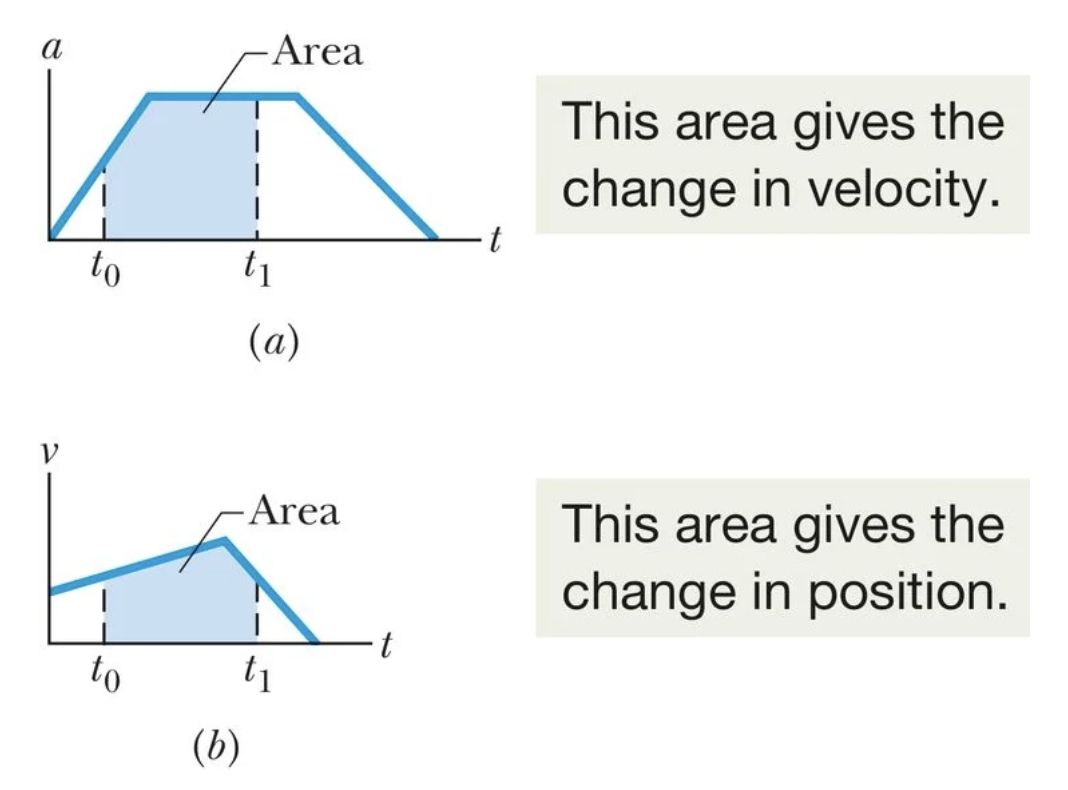
\includegraphics[scale=0.3]{area-under-curve}
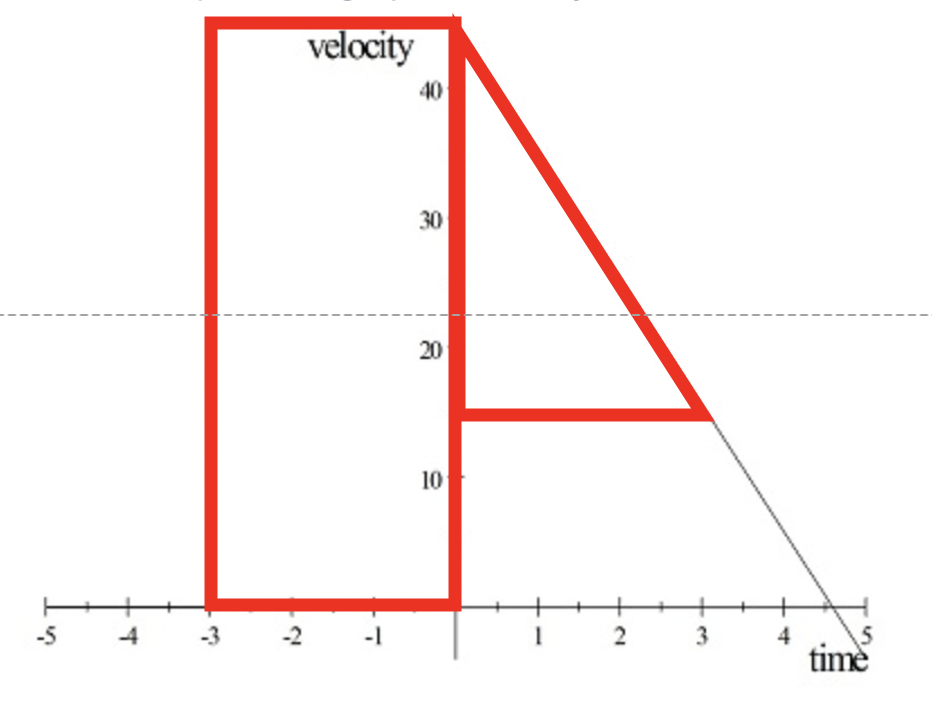
\includegraphics[scale=0.3]{area-under-curve-2}
\end{frame}


\begin{frame}{A example: whiplash curve}
\notsotiny
%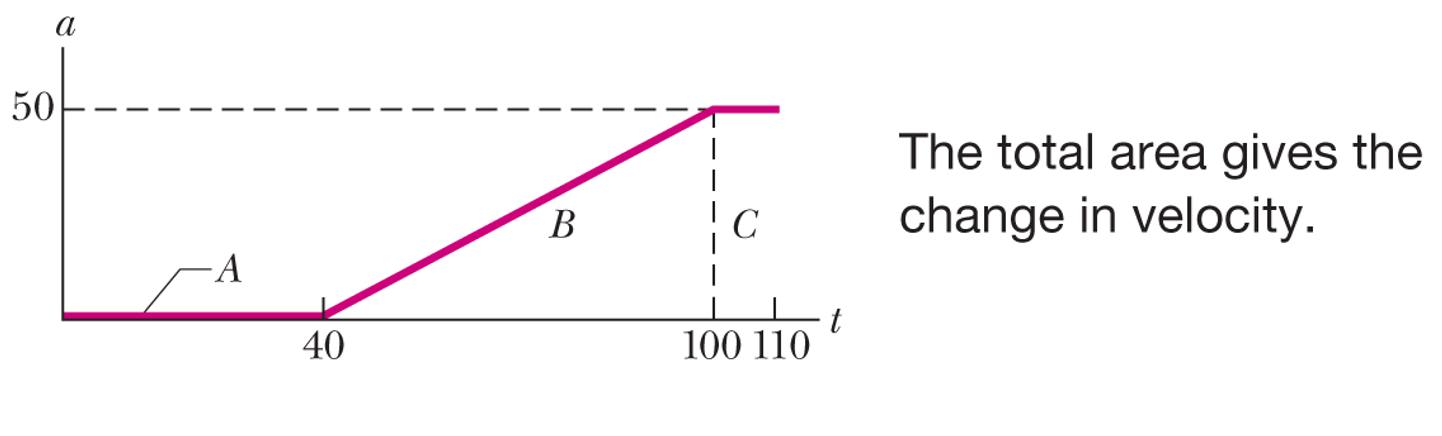
\includegraphics[scale=0.3]{whiplash1}

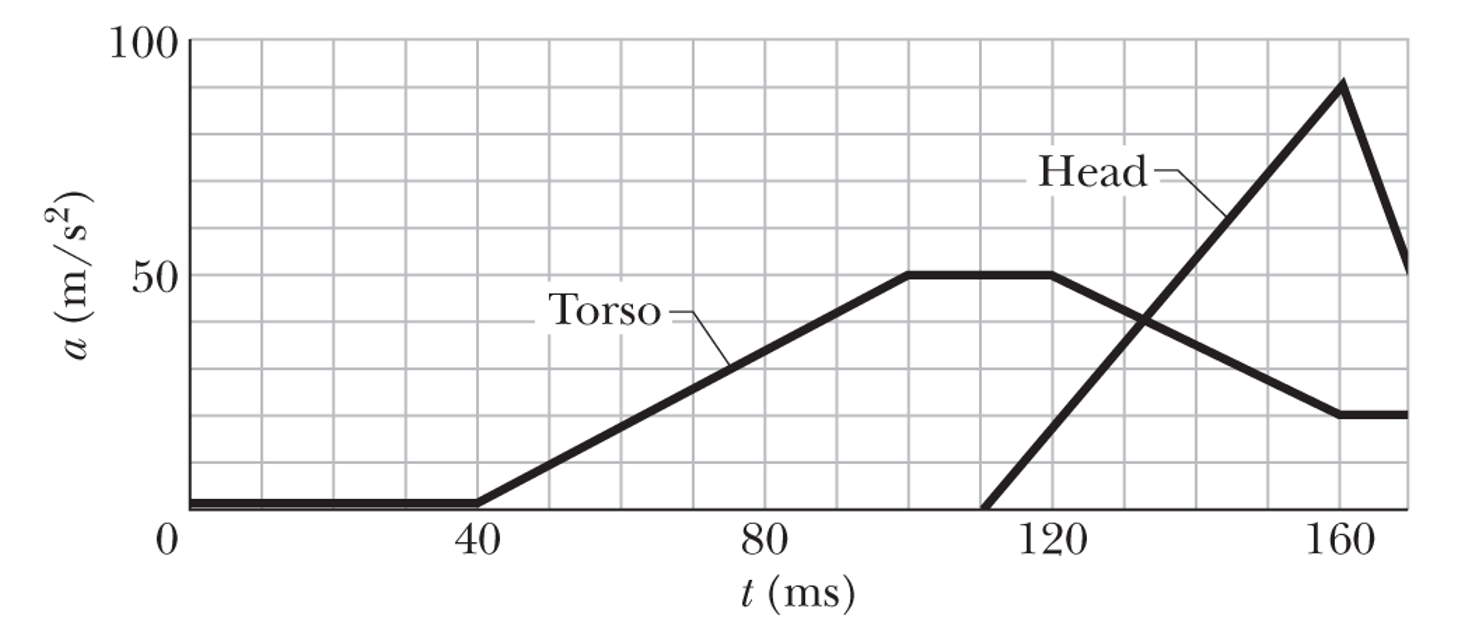
\includegraphics[scale=0.3]{whiplash2}
\end{frame}



\begin{frame}{Tackling confusion with directions}
\notsotiny
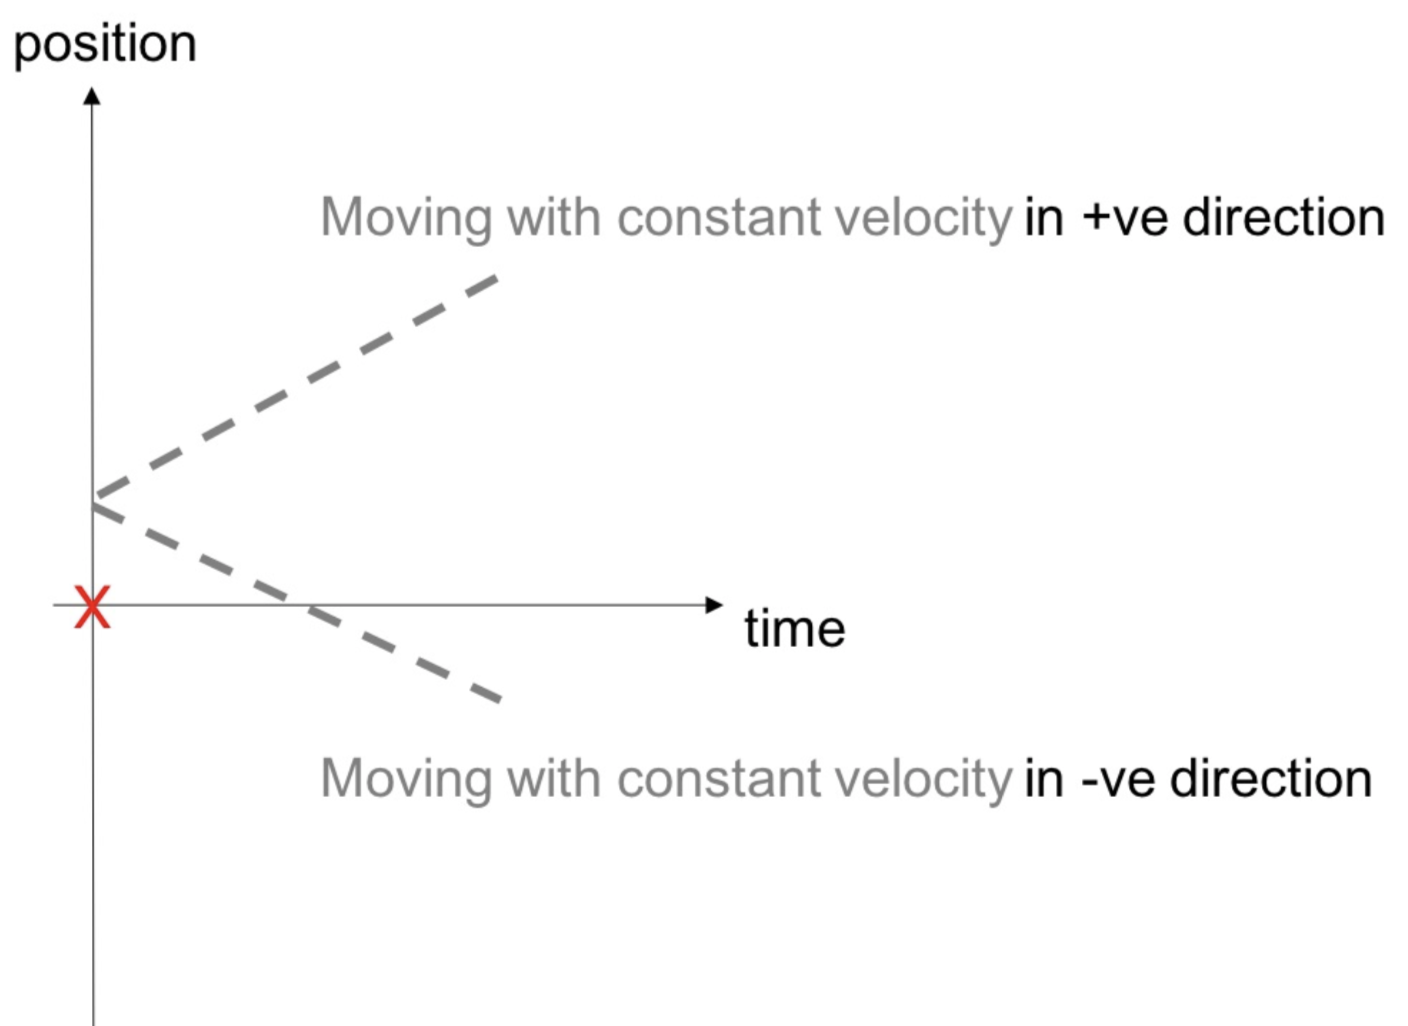
\includegraphics[scale=0.3]{PositionTime}

\end{frame}

\begin{frame}{Zero velocity is constant velocity}
\notsotiny
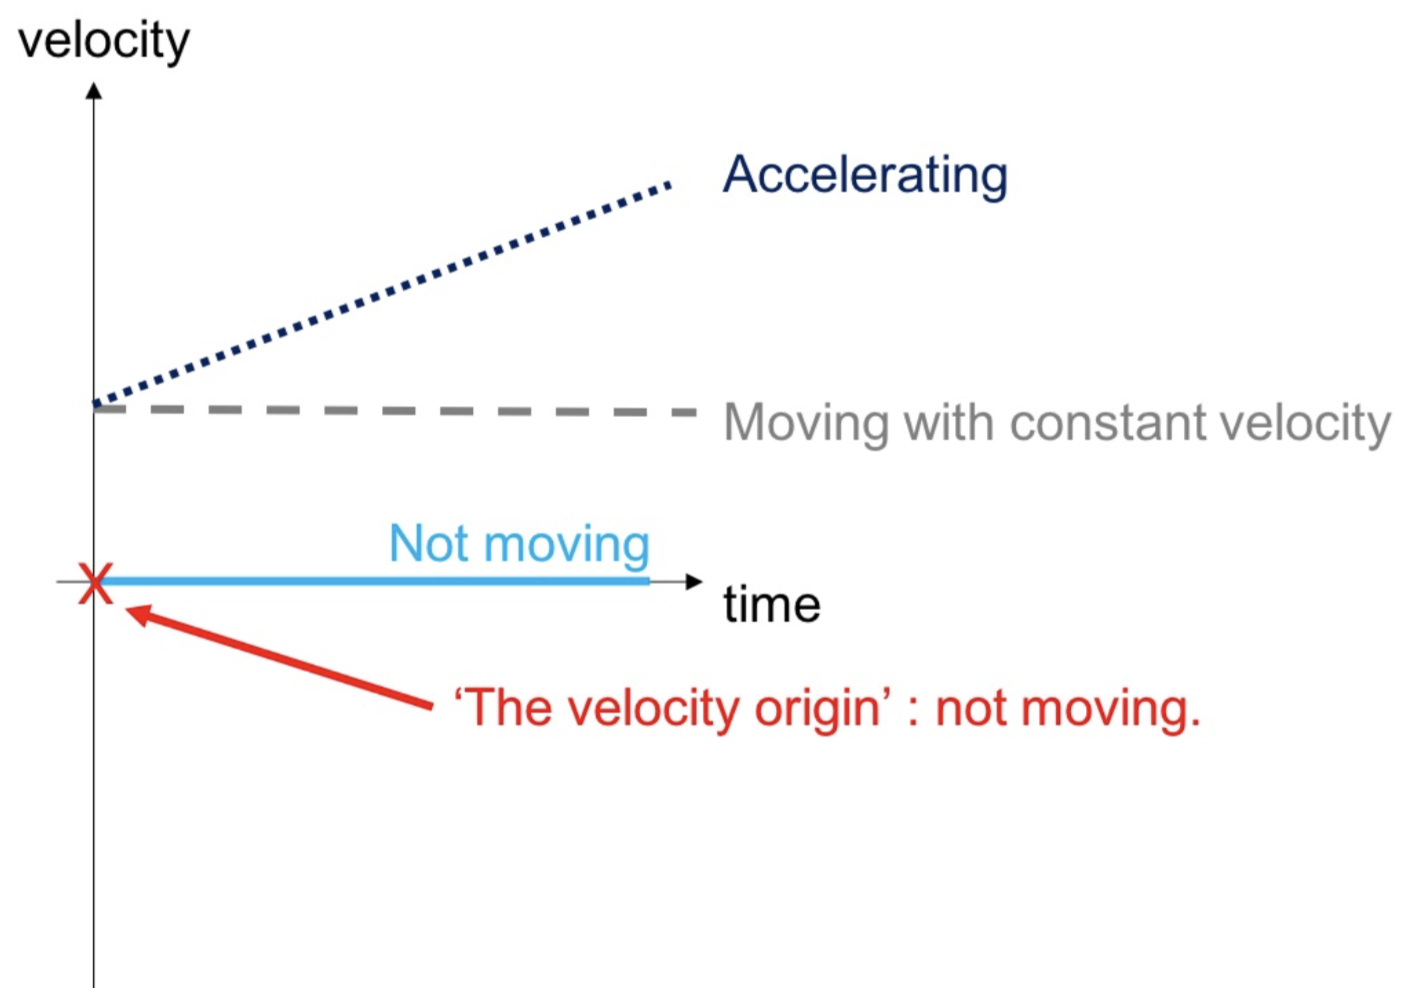
\includegraphics[scale=0.3]{VelocityTime}

\end{frame}


\begin{frame}{Matching slopes to values}
\notsotiny
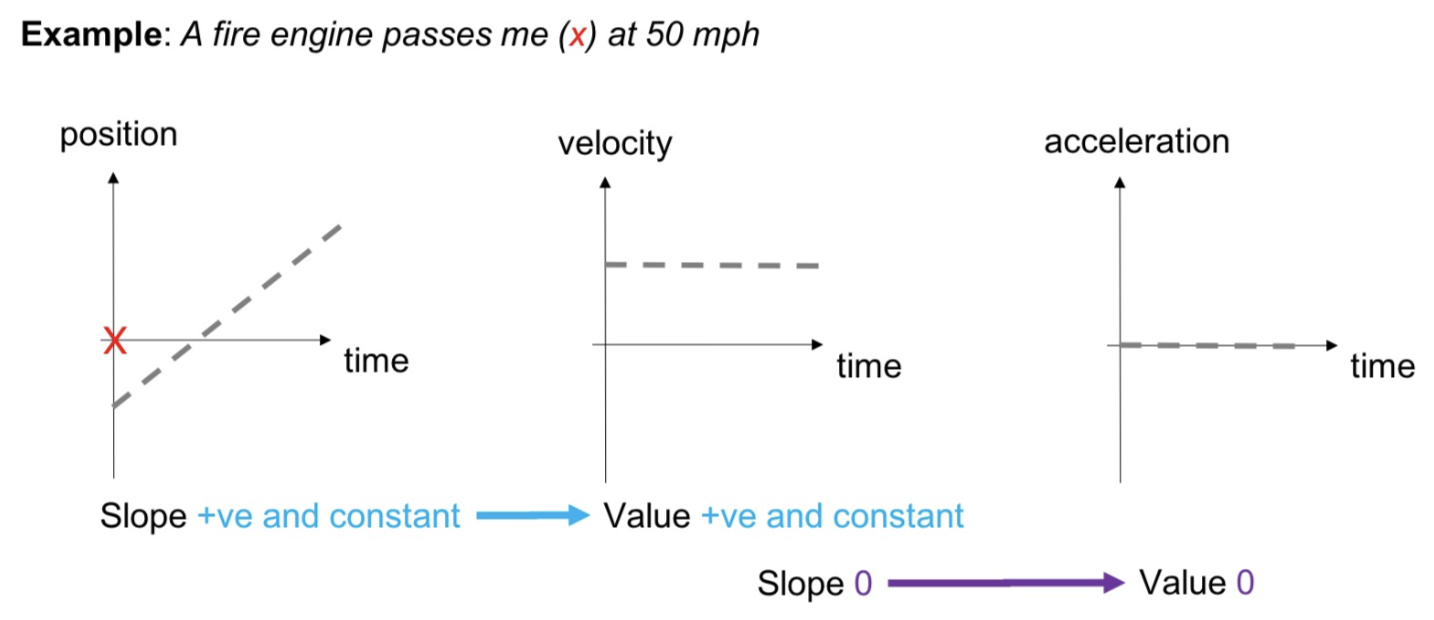
\includegraphics[scale=0.4]{FireEngine}

\end{frame}


\begin{frame}{A bouncing ball}
\small
How would we draw the motion of a ball being dropped from height, reaching ground, and bouncing back up again?\\
\vspace{5cm}

\end{frame}


\begin{frame}{Divide \& Conquer}
\notsotiny
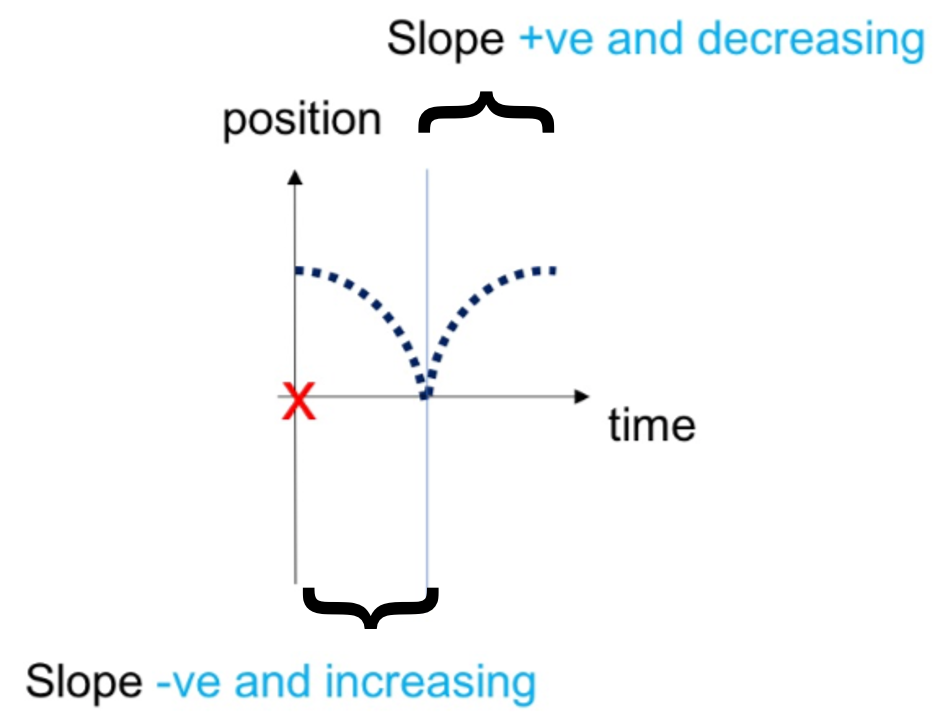
\includegraphics[scale=0.4]{ball1}

\end{frame}

\begin{frame}{Divide \& Conquer}
\notsotiny
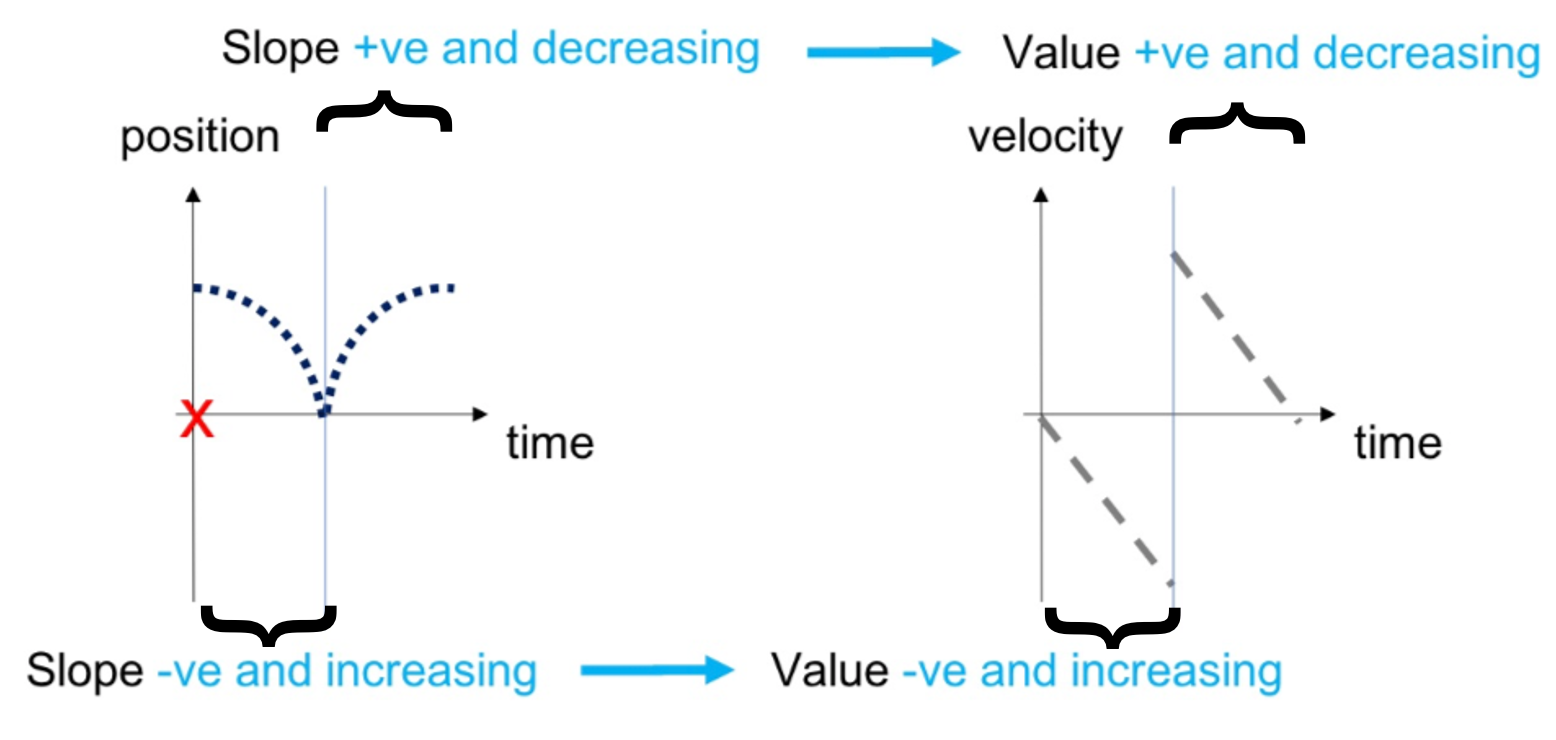
\includegraphics[scale=0.4]{ball2}

\end{frame}

\begin{frame}{Divide \& Conquer}
\notsotiny
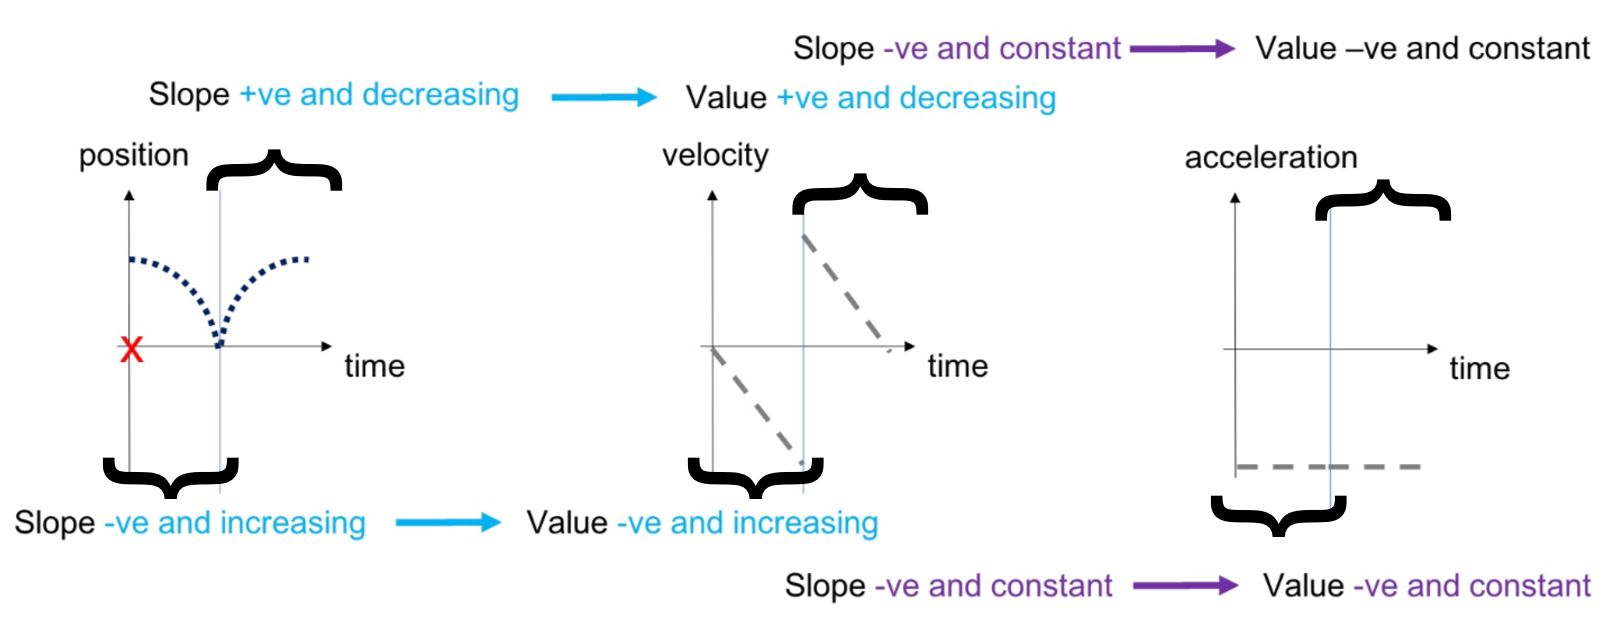
\includegraphics[scale=0.4]{ball3}

\end{frame}

\begin{frame}{Poll Everywhere Checkpoint (\textcolor{blue}{pollev.com/ilovephysics})}
\notsotiny
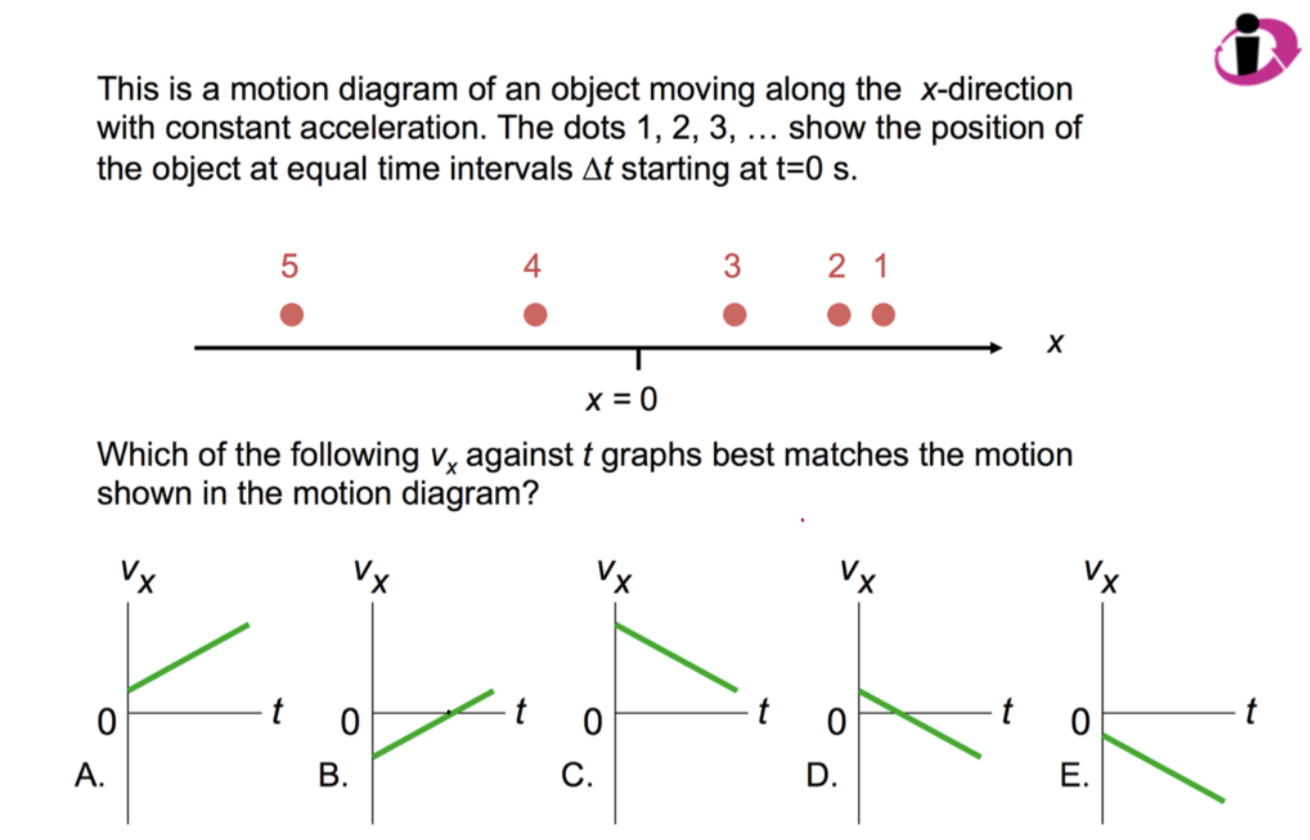
\includegraphics[scale=0.4]{GraphQuiz}

\end{frame}

\begin{frame}{Reading graphs: additional problem}
\notsotiny
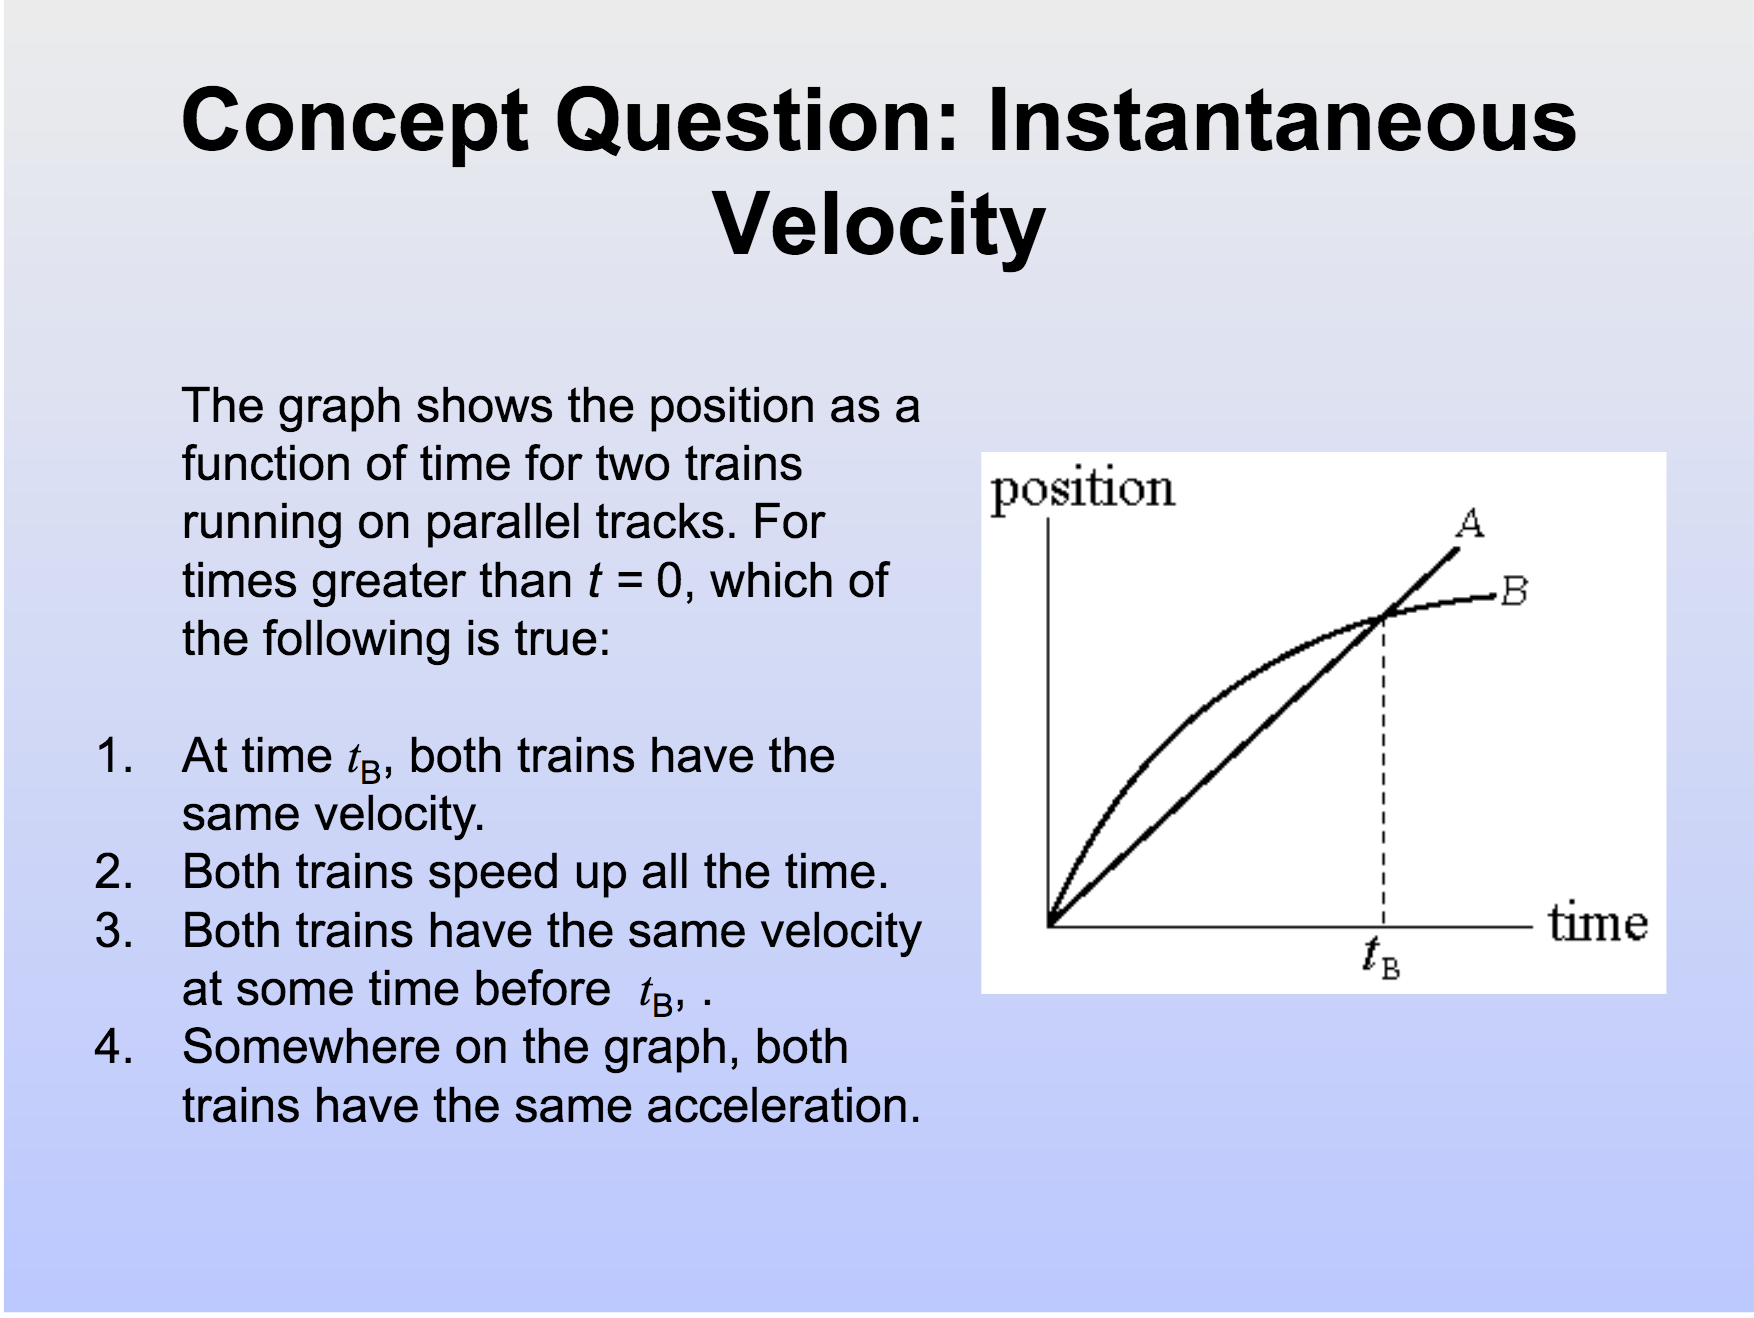
\includegraphics[scale=0.3]{NickedFromMIT}

\end{frame}



\begin{frame}{Preparing for next week's Kinematics Workshop}
\small
\begin{itemize}
\item The problems for the workshop are on Canvas.
\item Have a go at the problems prior to your workshop, so you know in advance what you would like the DT's help with.
\item Each workshop has a question marked out as the one you will be graded on.
\item Upload your solution to this before the end of next week.
\end{itemize}
\end{frame}

\begin{frame}{Tips}
\small
\begin{itemize}
\item You will need to use the quadratic formula at least once, so remind yourself what that is and when it is useful.
\item What information is given in the question? Write it down.
\item What information is known but not given? Write it down.
\item Underline or draw a box around your answer and take a photo of it (including working) and upload it to canvas.
\end{itemize}
\end{frame}
 
\end{document}